\section{Introducci\'on}

Los brazos robóticos articulados son sistemas mecánicos con articulaciones rotativas, diseñados para replicar funciones del brazo humano, incluyendo movimientos de rotación y alcance. Suelen tener una pieza en el extremo del robot llamado efector final, como se muestra en la Figura \ref{fig:brazoR}, que realiza la función del robot en el entorno (soldar, manipular objetos, etc.). Cada eje de movilidad en las uniones de las articulaciones representa un grado de libertad (DoF); de este modo, si una unión puede girar de izquierda a derecha, y de arriba hacia abajo, se dice que tiene dos DoF.

\vspace{1cm}

\begin{figure}[htb]
	\centering
	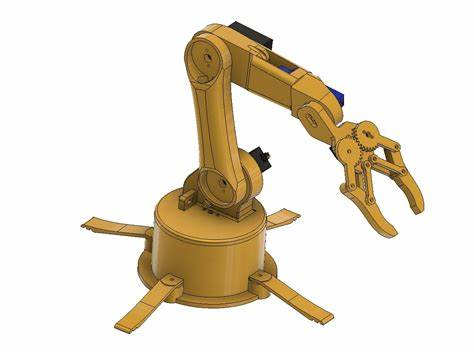
\includegraphics[scale=0.3]{brazo.jpeg}
	\caption{Partes de un brazo robótico articulado de 3 DoF}
	\label{fig:brazoR}
\end{figure}

\newpage
Sistemas Eléctricos de Potencia Computarizada (SEPDC) es una empresa mexicana que se dedica a fabricar la serie Kaab de Controladores Lógicos Programables (PLC), computadoras especializadas para la automatización industrial (tienen inmunidad al ruido eléctrico y resistencia a la vibración y al impacto). Cada uno de ellos puede ser operado de forma remota a través de un software llamado SettDev. En la Figura \ref{fig:plc} se muestra el PLC-Kaab.

\begin{figure}[htb]
	\centering
	\includegraphics[scale=0.9]{plckaab.png}
	\caption{PLC-Kaab fabricado por SEDPC}
	\label{fig:plc}
\end{figure}

Los PLC´s pueden ser empleados para el control de sistemas críticos, como lo demuestra la Figura \ref{fig:siscritico}. El termistor mide la temperatura en el ambiente; este valor es enviado al PLC, quien toma una decisión basado en dicho valor para controlar la apertura de una válvula por medio de un motor, dejando pasar cierta cantidad de líquido a través de la tubería.

\begin{figure}[htb]
	\centering
	\includegraphics[scale=0.9]{siscritico.png}
	\caption{Uso de un PLC para controlar un sistema crítico}
	\label{fig:siscritico}
\end{figure}